\section{Binomialkoeffizient}
\textbf{Definition:}  Der Binomialkoeffizient $\binom{n}{k}$ ist die Anzahl der k-elementigen Teilmengen von \{1,..,n\}\medskip\\
$$\text{\textbf{Formel: }}\binom{n}{k}= \frac{n*(n-1)*...*(n-k+1)}{k!}$$
$$=\frac{n!}{(n-k)!*k!}$$ mit k $\in$ \{0,...,n\}\medskip\\
\textbf{ Wieso teilen wir durch (k!)?}\\
Weil jede k-elementige Teilmenge k!-mal gezählt wurde. (z.B. \{3,5,9\} als (3,5,9), (3,9,5),...)\medskip\\
\textbf{Beispiel:} 20 Schüler.\\Es soll eine Fußballmanschafft gebildet werden.\\
Anzahl der Möglichkeiten ohne Berücksichtigung der Positionen: $\binom{20}{10}$\medskip\\
\textbf{Beispiel:} 52 Karten, davon 4 Asse. Wir ziehen 4 Karten ohne zurücklegen. Wahrscheinlichkeit, dass alle 4 Asse sind = ?\\
$\Omega$ = 4-elementige Teilmengen von \{1,...,52\}\\
\#A=1 \hspace{1cm} $\mathds{P}[A]=\dfrac{\#A}{\Omega}=\dfrac{1}{\binom{52}{4}}=3,7*10^{-6}$\medskip\\
\textbf{Beispiel:} 52 Karten, 4 werden gezogen.\\
A = ''Alle sind Pik''
$\mathds{P}[A]= ? \qquad \#A=\binom{13}{4} $\\
\#$\Omega = \binom{52}{4} \qquad \mathds{P}[A] = \dfrac{\binom{13}{4}}{\binom{52}{4}} \approx 2,64*10-{-3} $\\\\\\
\textbf{Satz 3.1:}\\ Wenn 0 $\leq$ k $\leq$n-1, dann gilt:
$\binom{n}{k}=\binom{n-1}{k}+\binom{n-1}{k-1}$\medskip\\
\textbf{Beweis:} Wir wollen aus n Elementen k auswählen.\\
Hier gibt es zwei Fälle:
\begin{enumerate}
	\item Wir haben das Element ''n'' ausgewählt. \\ Es verbleiben n-1 Elemente, von denen k-1 ausgewählt werden sollen.\\ $\implies \binom{n-1}{k-1}$ Möglichkeiten
	\item Wir haben das Element ''n'' nicht ausgewählt.\\
	Es verbleiben n-1 Elemente, von denen k ausgewählt werden sollen.\\ $\implies \binom{n-1}{k}$ Möglichkeiten
\end{enumerate}
\section{Binomischer Lehrsatz}
\begin{floatingfigure}[r]{6cm}
	\mbox{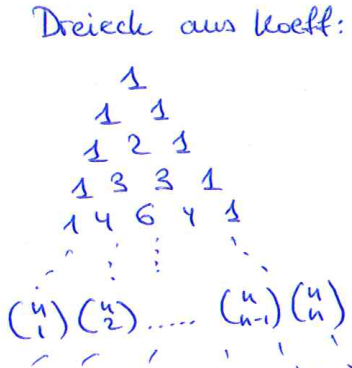
\includegraphics[width=0.3\textwidth]{img/pascal.PNG}}
	\caption{Pascalsches\\ Dreieck}
\end{floatingfigure}
$(x+y)^0=1$\\
$(x+y)^1 = x+y$\\
$(x+y)^2 = x^2+2xy+y^2$\\
$(x+y)^3= x^3+3x^2y+3xy^2+y^3$\medskip\\
$(x+y)^n=x^n+\binom{n}{1}x^{n-1}y+\binom{n}{2}x^{n-2}y^2+...+y^n$\medskip\\ 
\textbf{Satz 3.2.}:\\
$(x+y)^n =\sum^n_{k=0} \binom{n}{k}x^ky^{n-k}$\medskip\\
\textbf{Beweis}: \\
Beim Ausmultiplizieren zählen wir, wie oft der Term $x^ky^{n-k}$ entsteht.\\
Aus k Faktoren muss x als Beitrag ausgewählt werden, aus dem Rest y.
$(x+y)^n=(x+y)(x+y)*...*(x+y)$\\
$\binom{n}{k}$ Möglichkeiten \qed\medskip\\
\textbf{Bemerkung:} $\binom{n}{k}=\binom{n}{k-1}$, d.h. jede (Spalte vom Pascal'schen Dreieck) liest sich von rechts genauso wie von links.\\
k Elemente auswählen $\Leftrightarrow$ n-k nicht auswählen.\medskip\\
\textbf{Beobachtung}: Zeilen summieren im Pascal'schen Dreieck: Zeilen summieren im Pascal'schen Dreieck: Summe ist $2^n$\medskip\\
\textbf{Satz 3.3}: $\sum^n_{k=0} \binom{n}{k} = 2^n$\medskip\\
\textbf{Beweis}:\\
$\sum^n_{k=0}\binom{n}{k}1^k1^{n-k} = (1+1)^n=2^n\qed$\medskip\\
\textbf{Übung}: (ähnlich)\\
$\binom{n}{0}+\binom{n}{2}+\binom{n}{4}+...=\binom{n}{1}+\binom{n}{3}+\binom{n}{5}+...$\newpage
\subsection{Pascal'sches Dreieck und Trigonometrie}
\begin{tabbing}
	\textbf{Bekannt}: \= $\sin(2x) = 2\sin x \cos x$\\
	\> $\cos(2x)=\cos^2x-\sin^2x$
\end{tabbing}
Es gibt auch Formeln für $\sin(3x) , \cos(3x)$,...\smallskip\\
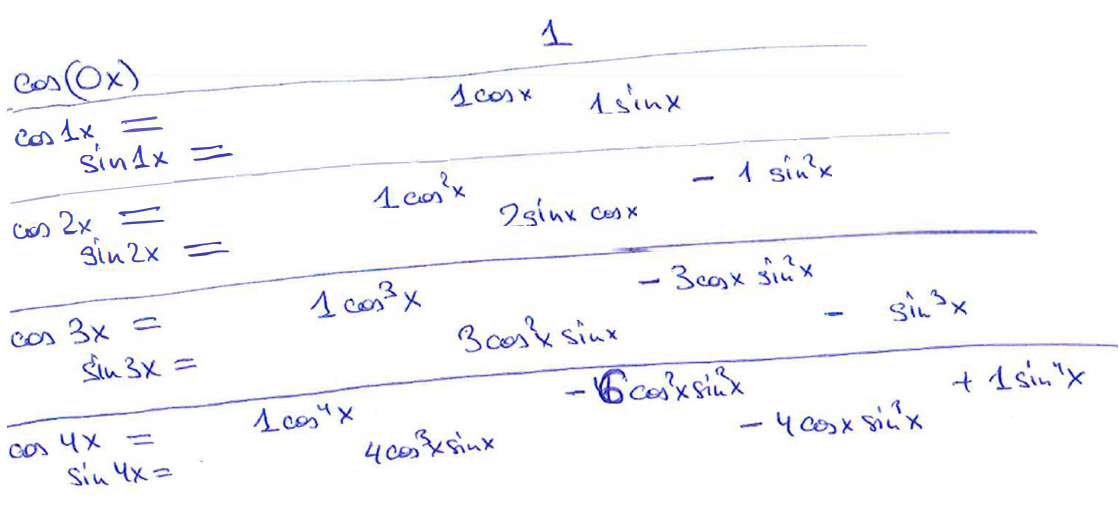
\includegraphics[width=0.8\textwidth]{img/ayy.PNG}\medskip\\
\textbf{Allgemein}:\\
$\sin(nx) = \binom{n}{1}\cos^{n-1}(x) \sin x - \binom{n}{3}\cos^{n-1}x \sin^3x + \binom{n}{5} \cos^{n-5}x \sin^5x-...$\medskip\\
$\cos(nx) = \cos^nx - \binom{n}{2}\cos^{n-2}x\sin^2x+\binom{n}{4}\cos^{n-4}x\sin^4x-...$\medskip\\
\textbf{Beweis}: Induktion (Übung YAAAY)
\section{Hypergeometrische Verteilung}
\begin{tabbing}
	Teich mit n Fischen:\hspace{1cm}\= $n_1$ Fische rot\\
	$n_1 + n_2 = n$ \>$n_2$ Fische gelb
\end{tabbing}
Fischer fängt k Fische (ohne Zurücklegen) mit k$\leq$n\medskip\\
A=''$k_1$ rote und $k_2$ gelbe Fische gefangen.''mit $k_1 + k_2 = k$\medskip\\
$\mathds{P}[A] = ?$\medskip\\
\textbf{Lösung:} $\Omega$ = \{T $\subseteq$ \{1,...,n\}, \#T = k\}\hspace{5mm} \#$\Omega=\binom{n}{k}$\medskip\\
Ereignis A = ''Aus $n_1$ roten Fischen $k_1$ auswählen $\binom{n_1}{k_1}$ und aus $n_2$ gelben Fischen $k_2$ auswählen $\binom{n_2}{k_2}$''\medskip\\
Diese sind beliebig kombinierbar.\medskip\\
Insgesamt: \#A = $\binom{n_1}{k_1}*\binom{n_2}{k_2}$\medskip\\
$\mathds{P}[A] = \dfrac{\binom{n_1}{k_1}*\binom{n_2}{k_2}}{\binom{n}{k}}$
\\\\\\\\\\
\textbf{Beispiel:} Lotto: 6 aus 49\medskip\\
Ereignis A = "Man hat genau 3 richtig"\medskip\\
$\mathds{P}$[A] = ?\medskip\\
\textbf{Lösung:}\\
$\Omega = \{T \subseteq \{1,...,49\},|T| = 6\} \qquad \#\Omega = \binom{49}{6}$\medskip\\
Ohne Einschränkung tippen wir auf \{1,...,6\} damit A eintritt:
\begin{itemize}
	\item Es müssen 3 Kugeln aus \{1,...,6\} gezogen werden: $\binom{6}{3}$ Möglichkeiten
	\item Es müssen 3 Kugeln aus \{7,...,49\} gezogen werden: $\binom{43}{3}$ Möglichkeiten\medskip\\
	\#A = $\binom{6}{3}*\binom{43}{3}$\smallskip\\
	$\mathds{P}[A] = \dfrac{\binom{6}{3}*\binom{43}{3}}{\binom{49}{6}}\approx 0,0176$
\end{itemize}
